
\textbf{Question 1}

Un lycéen ne répondra « oui » à la question « Avez-vous consommé du cannabis ? » que s'il a tiré un 6 lors d'un lancer de dé, soit avec une probabilité de :$\dfrac{1}{6}.
$

\textbf{Question 2}

\begin{center}
	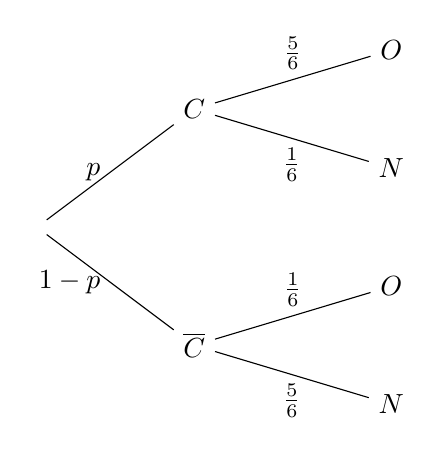
\begin{tikzpicture}
		[level 1/.style={level distance=2cm,
			sibling distance=3cm},
		level 2/.style={level distance=2.5cm,
			sibling distance=1.5cm}]
		\node {} [grow'=right]
		child {node {$C$}
			child {node {$O$}
				edge from parent node[above] {$\frac56$}
			}
			child {node {$N$}
				edge from parent node[below] {$\frac16$}
			}
			edge from parent node[left] {$p$}
		}
		child {node {$\overline C$}
			child {node {$O$}
				edge from parent node[above] {$\frac16$}
			}
			child {node {$N$}
				edge from parent node[below] {$\frac56$}
			}
			edge from parent node[left ] {$1-p$}
		}
		;
	\end{tikzpicture}
\end{center}

\textbf{Question 3}

\begin{align*}
	p(C \cap O) &= p(C) \times p_C(O) = p \times \dfrac{5}{6} = \dfrac{5p}{6}, \\
	p(\overline{C} \cap O) &= p(\overline{C}) \times p_{\overline{C}}(O) = (1 - p) \times \dfrac{1}{6} = \dfrac{1 - p}{6}.
\end{align*}

D'après la loi des probabilités totales :
\[
p(O) = p(C \cap O) + p(\overline{C} \cap O) = \dfrac{5p}{6} + \dfrac{1 - p}{6} = \dfrac{4p + 1}{6}.
\]

\textbf{Question 4}

Pour le calcul de $p_N(C)$, on utilise la formule de Bayes :
\[
p_N(C) = \dfrac{p(C \cap N)}{p(N)} = \dfrac{0,35 \times \dfrac{5}{6}}{1 - \dfrac{3}{5}} = \dfrac{35}{48}.
\]


